% Template for Elsevier CRC journal article
% version 1.1 dated 16 March 2010

% This file (c) 2010 Elsevier Ltd.  Modifications may be freely made,
% provided the edited file is saved under a different name

% This file contains modifications for Procedia Computer Science
% but may easily be adapted to other journals

% Changes since version 1.0
% - elsarticle class option changed from 1p to 3p (to better reflect CRC layout)

%-----------------------------------------------------------------------------------

%% This template uses the elsarticle.cls document class and the extension package ecrc.sty
%% For full documentation on usage of elsarticle.cls, consult the documentation "elsdoc.pdf"
%% Further resources available at http://www.elsevier.com/latex

%-----------------------------------------------------------------------------------

%%%%%%%%%%%%%%%%%%%%%%%%%%%%%%%%%%%%%%%%%%%%%%
%%%%%%%%%%%%%%%%%%%%%%%%%%%%%%%%%%%%%%%%%%%%%%
%%                                          %%
%% Important note on usage                  %%
%% -----------------------                  %%
%% This file must be compiled with PDFLaTeX %%
%% Using standard LaTeX will not work!      %%
%%                                          %%
%%%%%%%%%%%%%%%%%%%%%%%%%%%%%%%%%%%%%%%%%%%%%%
%%%%%%%%%%%%%%%%%%%%%%%%%%%%%%%%%%%%%%%%%%%%%%

%% The '3p' and 'times' class options of elsarticle are used for Elsevier CRC
\documentclass[3p,times]{elsarticle}

%% The `ecrc' package must be called to make the CRC functionality available
%\usepackage{ecrc}

%% The ecrc package defines commands needed for running heads and logos.
%% For running heads, you can set the journal name, the volume, the starting page and the authors

%% set the volume if you know. Otherwise `00'
%\volume{00}

%% set the starting page if not 1
%\firstpage{1}

%% Give the name of the journal
%\journalname{}

%% Give the author list to appear in the running head
%% Example \runauth{C.V. Radhakrishnan et al.}
%\runauth{}

%% The choice of journal logo is determined by the \jid and \jnltitlelogo commands.
%% A user-supplied logo with the name <\jid>logo.pdf will be inserted if present.
%% e.g. if \jid{yspmi} the system will look for a file yspmilogo.pdf
%% Otherwise the content of \jnltitlelogo will be set between horizontal lines as a default logo

%% Give the abbreviation of the Journal.
%\jid{procs}

%% Give a short journal name for the dummy logo (if needed)
%\jnltitlelogo{}

%% Hereafter the template follows `elsarticle'.
%% For more details see the existing template files elsarticle-template-harv.tex and elsarticle-template-num.tex.

%% Elsevier CRC generally uses a numbered reference style
%% For this, the conventions of elsarticle-template-num.tex should be followed (included below)
%% If using BibTeX, use the style file elsarticle-num.bst

%% End of ecrc-specific commands
%%%%%%%%%%%%%%%%%%%%%%%%%%%%%%%%%%%%%%%%%%%%%%%%%%%%%%%%%%%%%%%%%%%%%%%%%%

%% The amssymb package provides various useful mathematical symbols
\usepackage{amssymb}
%% The amsthm package provides extended theorem environments
\usepackage{amsthm}
\usepackage{amsmath}
\usepackage[section] {placeins}
%% The lineno packages adds line numbers. Start line numbering with
%% \begin{linenumbers}, end it with \end{linenumbers}. Or switch it on
%% for the whole article with \linenumbers after \end{frontmatter}.
%% \usepackage{lineno}

%% natbib.sty is loaded by default. However, natbib options can be
%% provided with \biboptions{...} command. Following options are
%% valid:

%%   round  -  round parentheses are used (default)
%%   square -  square brackets are used   [option]
%%   curly  -  curly braces are used      {option}
%%   angle  -  angle brackets are used    <option>
%%   semicolon  -  multiple citations separated by semi-colon
%%   colon  - same as semicolon, an earlier confusion
%%   comma  -  separated by comma
%%   numbers-  selects numerical citations
%%   super  -  numerical citations as superscripts
%%   sort   -  sorts multiple citations according to order in ref. list
%%   sort&compress   -  like sort, but also compresses numerical citations
%%   compress - compresses without sorting
%%
% \biboptions{comma,round}

 \biboptions{compress}
\usepackage{color}
\def\red#1{{\color{red}{#1}\color{black}}}
% if you have landscape tables
\usepackage[figuresright]{rotating}
\usepackage{amssymb}
% put your own definitions here:
%\newcommand{\eqref}{Ref.}
%   \newtheorem{def}{Definition}[section]
%   ...
\newfont{\fp}{msbm10 at 11pt}  
\def\E{\mbox{\fp E}}
\def\proof{\mbox{\fp Proof:}}
\newtheorem{prop}{Proposition}
\newtheorem{thm}{Theorem}
\usepackage[T1]{fontenc}
\usepackage{amsfonts}
\newtheorem{lem}{Lemma}
% add words to TeX's hyphenation exception list
%\hyphenation{author another created financial paper re-commend-ed Post-Script}

% declarations for front matter

\usepackage{color, colortbl, framed}

\begin{document}

\begin{frontmatter}

%% Title, authors and addresses

%% use the tnoteref command within \title for footnotes;
%% use the tnotetext command for the associated footnote;
%% use the fnref command within \author or \address for footnotes;
%% use the fntext command for the associated footnote;
%% use the corref command within \author for corresponding author footnotes;
%% use the cortext command for the associated footnote;
%% use the ead command for the email address,
%% and the form \ead[url] for the home page:
%%
%% \title{Title\tnoteref{label1}}
%% \tnotetext[label1]{}
%% \author{Name\corref{cor1}\fnref{label2}}
%% \ead{email address}
%% \ead[url]{home page}
%% \fntext[label2]{}
%% \cortext[cor1]{}
%% \address{Address\fnref{label3}}
%% \fntext[label3]{}

%\dochead{}
%% Use \dochead if there is an article header, e.g. \dochead{Short communication}
\title{The local maxima method for enhancement of time-frequency map and its application to local damage detection in rotating machines}

%% use optional labels to link authors explicitly to addresses:
%% \author[label1,label2]{<author name>}
%% \address[label1]{<address>}
%% \address[label2]{<address>}

%\author[lab1]{Jakub Obuchowski},  \author{lab2}{Agnieszka Wy{\l}oma{\'n}ska}, \author{lab1}{Rados{\l}aw Zimroz}

%\adress{lab1}{Diagnostics and Vibro-Acoustics Science Laboratory, Pl Teatralny 2, 50-051 Wroclaw, Wroclaw University of Technology, PL}\\
% \adress{lab2}{Hugo Steinhaus Center, Institute of Mathematics and Computer Science, Wroclaw University of Technology, PL} \\
 %\ead{       jakub.obuchowski@pwr.wroc.pl}\\
  %  radoslaw.zimroz@pwr.wroc.pl\\
   % agnieszka.wylomanska@pwr.wroc.pl
 %\author{Jakub Obuchowski, Agnieszka Wy{\l}oma{\'n}ska, Rados{\l}aw Zimroz}
 %\tnotetext[label1]{}
 \author{Jakub Obuchowski\fnref{label1}}
  %\ead{jakub.obuchowski@pwr.wroc.pl}
 % \tnotetext[label2]{}
\author{Agnieszka Wy{\l}oma{\'n}ska\fnref{label2}}
 %\ead{agnieszka.wylomanska@pwr.wroc.pl}
 %\tnotetext[label3]{}
   \author{Rados{\l}aw Zimroz\fnref{label1}}
  %  \ead{radoslaw.zimroz@pwr.wroc.pl}
%% \ead[url]{home page}\fntext[label2]{}
   \fntext[label1]{Diagnostics and Vibro-Acoustics Science Laboratory, Na Grobli 15, 50-421 Wroclaw, Wroclaw University of Technology, PL\\jakub.obuchowski@pwr.wroc.pl. radoslaw.zimroz@pwr.wroc.pl}
  \fntext[label2]{Hugo Steinhaus Center, Institute of Mathematics and Computer Science, Janiszewskiego 14 a, 50-370 Wroclaw, Wroclaw University of Technology, PL\\
   agnieszka.wylomanska@pwr.wroc.pl}
 
\begin{abstract}
In this paper a new method of fault detection in rotating machinery is presented. It is based on a vibration time series analysis in time-frequency domain. A raw vibration signal is decomposed via the short-time Fourier transform (STFT). Time-frequency map is considered as matrix ($M x N$) with N sub-signals with length M. Each sub-signal is considered as a time series and might be interpreted as energy variation for narrow frequency bins. Each sub-signal is processed using novel approach called the local maxima method. Basically we search for local maxima because they should appear in the signal if local damage in bearings or gearbox exists.  Finally, information for all sub-signals is combined in order to validate impulsive behavior of energy. Due to random character of obtained time series, each maximum occurrence has to be checked for its significance. If there are time points for which the average number of local maxima for all sub-signals is significantly higher than for the other time instances, then location of these maxima is "weighted" as more important (at this time instance local maxima create for set of $\Delta f$ a pattern on the time-frequency map). This information, called vector of weights is used for enhancement of spectrogram. When vector of weights is applied for spectrogram, non-informative energy is suppresed while informative features on spectrogram are enhanced. If distribution of local maxima on spectrogram creates a pattern of wide-band cyclic energy growth, the machine is suspected of being damaged.  For healthy condition, the vector of average number of maxima for each time point should not have outliers, aggregation of information from all sub-signals is rather random and does not create any pattern. The method is illustrated by analysis of very noisy both real and simulated signals.
\end{abstract}
\begin{keyword}
time-frequency analysis \sep enhancement \sep feature extraction \sep local maxima \sep local damage
%% keywords here, in the form: keyword \sep keyword

%% MSC codes here, in the form: \MSC code \sep code
%% or \MSC[2008] code \sep code (2000 is the default)

\end{keyword}
\end{frontmatter}
\section{Introduction}
In this paper a new method of localized damage detection in rotating machinery is presented. The most frequent medium for such damage detection is still vibration signal (acceleration),~\cite{bib1,bib2}. The basis for localized damage detection is the assumption that two surfaces being in touch (rolling element and inner/outer race, two teeth from gear-pair etc.) during sliding/rolling generate shocks due to damage of one of the surfaces. Such local change of stiffness results in singularity in the signal. From theoretical point of view, one should expect impulse in time domain for time instance when damaged part is in contact. For rotating machines (gears, bearings) signature of local damage is series of impulses with period (or more general cycle) related to so called fault frequency,~\cite{bib28}.\\
One might consider a diagnostic scheme: i) detect impulsive nature of the signal, ii) check if there is periodic nature of disturbance and try to match it to expected fault frequencies in the machine. Unfortunately, in practice, such cyclic impulse train can be hardly seen. There are two main possible reasons. First, one might not see impulses due to weakness of such disturbance and level of noise present during experiment -- this case is called "detection of damage at early stage". Second, damage is in developed form, however, due to high level of noise coming from other part of machine or other machines, diagnostic information is completely masked/hidden.\\
From methodological point of view, the problem is the same for both cases. One needs to "extract" informative signal from mixture of signals coming from different sources,~\cite{bib2,bib3,bib4,bib5,bib6,bib7,bib14,bib15,bib16,bib19,bib20,bib21,bib22,bib23,bib26,bib27}. By "noise" in such context one might consider narrowband contribution (discrete frequencies) coming from shaft, mesh, resonance, ghost, etc. components, wide-band Gaussian noise, or other. The most reasonable approach is to design filter, that would be able to extract signal of interest,~\cite{bib19,bib20,bib21,bib22,bib23,bib17,bib18}. However, the task could be also defined as "information" extraction (not exactly "signal", that contains information). In such a context one might model the signal, or try to analyze properties of the signal using another signal representation.\\
In the paper a raw vibration signal is decomposed via the short-time Fourier transform. Time-frequency representation is very reasonable method of non-stationary signal analysis,~\cite{bib14,bib15,bib16,bib8,bib9,bib10,bib11,bib12,bib13,HeManifold}. The STFT method is the simplest, the most intuitive for engineers and it will be used in the paper to present the algorithm,~\cite{bib8}. However, it should be said that there is no objection to apply proposed approach to another time-frequency representation as Wigner-Ville or time-scale~\cite{WangScale} one.\\
When signal is represented by STFT time-frequency plane, it can be interpreted as energy flow in time for set of frequency bins $\Delta f$. One might expect, that due to damage related shocks, impulses invisible in time domain will be present in time frequency plane, as a wide-band (for family of frequency bins $\Delta f$) disturbances occurred in cyclic way. Unfortunately, when signal to noise ratio is really poor (amplitudes of impulses are small in comparison to energy of non-informative sources) changes of energy are too small to be seen on the map clearly.\\
In practice, even time-frequency representation of complex signal may require some extra activities, i.e. enhancement of time-frequency plane readability before feature extraction and decision making. This is the case for analysed signals. It has given "an impulse" for searching a way to "enhance" time-frequency map and "extract" information about cyclic, impulsive behavior at some frequency range.\\
In this paper a novel method of spectrogram enhancement and extraction information required for local damage detection in rotating machinery is proposed. The basic idea comes from interpretation of STFT map as a set of sub-signals (one signal for frequency bin $\Delta f$) with much smaller complexity and application of simple tools as local maxima finder for each sub-signal separately. Local maxima are searched because local increase of energy is expected when damage occurs. So basically it can be said that signal is "decomposed" into set of sub-signals, each sub-signal is processed/analysed in order to check if for investigated frequency bin $\Delta f$ an impulsive energy exists and finally information for all sub-signals is fused in order to validate impulsive behavior of energy. Local maxima finder is looking for local maximum value of sub-signal in short moving window. It might happen, that as results one might obtain set of random maxima. So, due to random character of obtained time series, each maximum occurrence must be checked for its significance. \\
Validation of local maxima detection is done by comparison of results obtained for different sub-signals. If there are time points for which the average number of local maxima for all sub-signals is significantly higher than for the other time instances, then location of these maxima is "weighted" as more important (this time instance creates a pattern on the time-frequency map).\\
This information, called vector of weights is used for enhancement of spectrogram. When vector of weights is applied for spectrogram, non-informative energy is suppressed while informative features on spectrogram are enhanced. If distribution of local maxima on spectrogram creates a pattern on wideband cyclic energy growth the machine is suspected of being damaged. For healthy condition, the vector of average number of maxima for each time point should not have outliers, aggregation of information from all subsignals is rather random and does not create any pattern. The method is illustrated by analysis of very noisy both real and simulated signals.\\
The paper is organized as follows: in Sec.~\ref{methodology} a proposal of new time-frequency map enhancement procedure is presented. Sec.~\ref{simulated} contains analysis of simulated data according to the presented procedure. In Sec.~\ref{experiment} we describe the experiment while in Sec.~\ref{real} we present the results for the described real data. In Section~\ref{discussion} we present the discussion and last section contains conclusions.
\section{Methodology}\label{methodology}
In this section we present in details  the local maxima method which was previously based on non-overlapping windows in short time Fourier transform~\cite{bib3}. Here we describe how to adapt it to highly-overlapping windows.
The local maxima method starts with a transformation which converts a signal in time domain into a two-dimensional map (time-frequency), where spikes in time domain become wide-band excitations. In this paper we use the short-time Fourier transform that is denoted by $\{STFT(t,f)\}_{t\in T, f\in F}$, where $T$ is the set of time points and $F$ stands for the set of frequencies for which the transform is calculated. In the further analysis we assume $T=\{t_1,....,t_{\#T}\}$, where $\#T$ denotes number of elements of the set $T$. The STFT for random sample $X_1, ...,X_n$, time point $t_i$ and frequency $f$ is defined as follows:
\begin{eqnarray}
STFT(t_i,f)=\sum_{k=1}^{n}X_k\tilde{W}_{k-t_i}e^{jfk},
\end{eqnarray}
where $\{\tilde{W}_k\}$ is the window sequence.\\
Once the map is obtained, time series related to each $f\in F$ are analyzed.  For a given $f\in F$  and $t_i$ we put $M(t_i,f)=1$ if $|STFT(t_i,f)|=max\{|STFT(t_k,f)|: i-r\leq k\leq i+r\}$ and $M(t_i,f)=0$ elsewhere. The binary spectrogram obtained by applying this rule for every time series should have clearly visible wide-band excitations with small amount of local maxima between them if $r$ is properly chosen. We suggest  that $r$ (called the minimal neighborhood length) should be as high as it is possible to theoretically preserve all the cyclic wide-band excitations related to damage in a rotating machine. In the non-overlapping windows case $r$ is calculated as the highest integer value not greater than ratio of the expected time between the following disturbances to the STFT window length, both expressed in the same units, i.e. in samples or in a unit of time. The formula for $r$ is:
\begin{eqnarray}\label{row1}r=\left\lfloor (fs/ff)/Nw-1\right\rfloor
\end{eqnarray}
where $fs$ is the sampling frequency, $ff$ is the fault frequency, $Nw$ stands for the STFT window length and $\lfloor x\rfloor$ is the largest integer not greater than $x$. In the overlapping windows case we propose to modify equation (\ref{row1}) as follows:
\begin{eqnarray}\label{row2}
r=\left\lfloor ((fs/ff)/Nw-1)/(1-Ov)\right\rfloor,
\end{eqnarray}
where $Ov$ denotes overlap ratio, i.e. the ratio of the number of samples that each window overlaps to the window length. In the further analysis we use $Ov=0.95$ and compare it to $Ov=0$. In practice, there might be some deviations from the theoretical distance between local maxima. To illustrate this point, consider series of impulses of different height. It can be caused both by random character of shocks and random background noise. Relaxation of the impulses, even in local damage case, takes a little of time so the real distance between local maxima in a particular time series might be a little smaller than theoretical. Moreover, some of rotating machines exhibit jitter (e.g. bearings) during operation under constant rotational speed, so the real distance might be a little higher or lower than the distance obtained by using equation (\ref{row2}).\\
The next step in our procedure is to calculate the vector of weights and combine it with the binary spectrogram obtaining the enhanced spectrogram. The latter one is formulated as follows:
\begin{eqnarray}\label{row3}
ENH(t_i,f)=W(t_i)M(t_i,f),
\end{eqnarray}
where $W(t_i)=\frac{1}{\#F}\sum_{f\in F}M(t_i,f)$ is the vector of weights and $M(t_i,f)$  represents binary valued time series of the local maxima occurrence
for a time point  $t_i$ and frequency $f$. Conversion of the time-frequency map $\{|STFT(t,f)|\}_{t\in T, f\in F}$ into the binary matrix $\{M(t,f)\}_{t\in T, f\in F}$ preserves energy-invariance, i.e. local maxima in a low-energy frequency bin are as significant as local maxima in other frequency bin. An impulse in the vector of weights calculated as average value of $\{M(t_i,f)\}_{f\in F}$, for a particular time $t_i$ is present only if there is a significant number of local maxima at $t_i$, i.e. larger than in the case where local maxima at $t_i$ are the result of random character of the signal. If there are no wideband exciatations in the time-frequency map or frequency bands of the excitations are not significantly wide then the vector of weights has no pulses. Thus, in locally damaged machine case the enhanced time frequency map increases visibility of wideband excitations and decreases influence of high-energy components. In healthy machine case it presents time-frequency map without any pattern. Moreover, arithmetic mean in the formula for $W(t_i)$ makes the result invariant to number of points at which FFT is calculated.\\
In the next step of our procedure we propose to analyze the enhanced version of vector of weights, i.e. vector calculated as follows:
\begin{eqnarray}\label{row4}
V(t_i)=\frac{1}{\#F}\sum_{f\in F}ENH(t_i,f).
\label{enh_VoW}\end{eqnarray}
Formula~\ref{enh_VoW} reduces noise present in $\{W(t)\}_{t\in T}$ putting highes values to time points at which the enhanced spectrogram $\{ENH(t,f)\}_{t\in T, f\in F}$ has wideband excitations instead of taking into account only binary matrix $\{M(t,f)\}_{t\in T, f\in F}$ (as in $\{W(t)\}_{t\in T}$).\\
One of the tool useful to estimate the fault frequency is the sample autocorrelation function (ACF). For a random sample $Y_1,Y_2,...,Y_n$ the ACF  it is defined as follows:
\begin{eqnarray}
R(k)=\frac{\sum_{i=1}^{n-|k|}(Y_i-\bar{Y})(Y_{i+k}-\bar{Y})}{\sqrt{\sum_{i=1}^n(Y_i-\bar{Y})^2}},
\end{eqnarray}
where $\bar{Y}$ is a sample mean of the random sample $Y_1,Y_2,...,Y_n$. The vector of weights (and its enhanced version) is a set of non-negative real numbers including a set of significantly higher values in the case of local damage. If time intervals between these values are equal, then the sample ACF should be higher at lags related to them. It was shown that even in the case of poor resolution on time scale the sample ACF is sufficient to estimate the fault frequency.\\
The main purpose to use overlapping windows is better resolution on time scale. In this paper it will be examined whether the sample ACF will still be useful in the case of better time resolution. What is more, this examination will be preceded by analysis of envelope spectra in both overlapping and non-overlapping cases.\\
The whole procedure is presented in Fig.~\ref{fig01}
\begin{figure}[ht]
\begin{center}
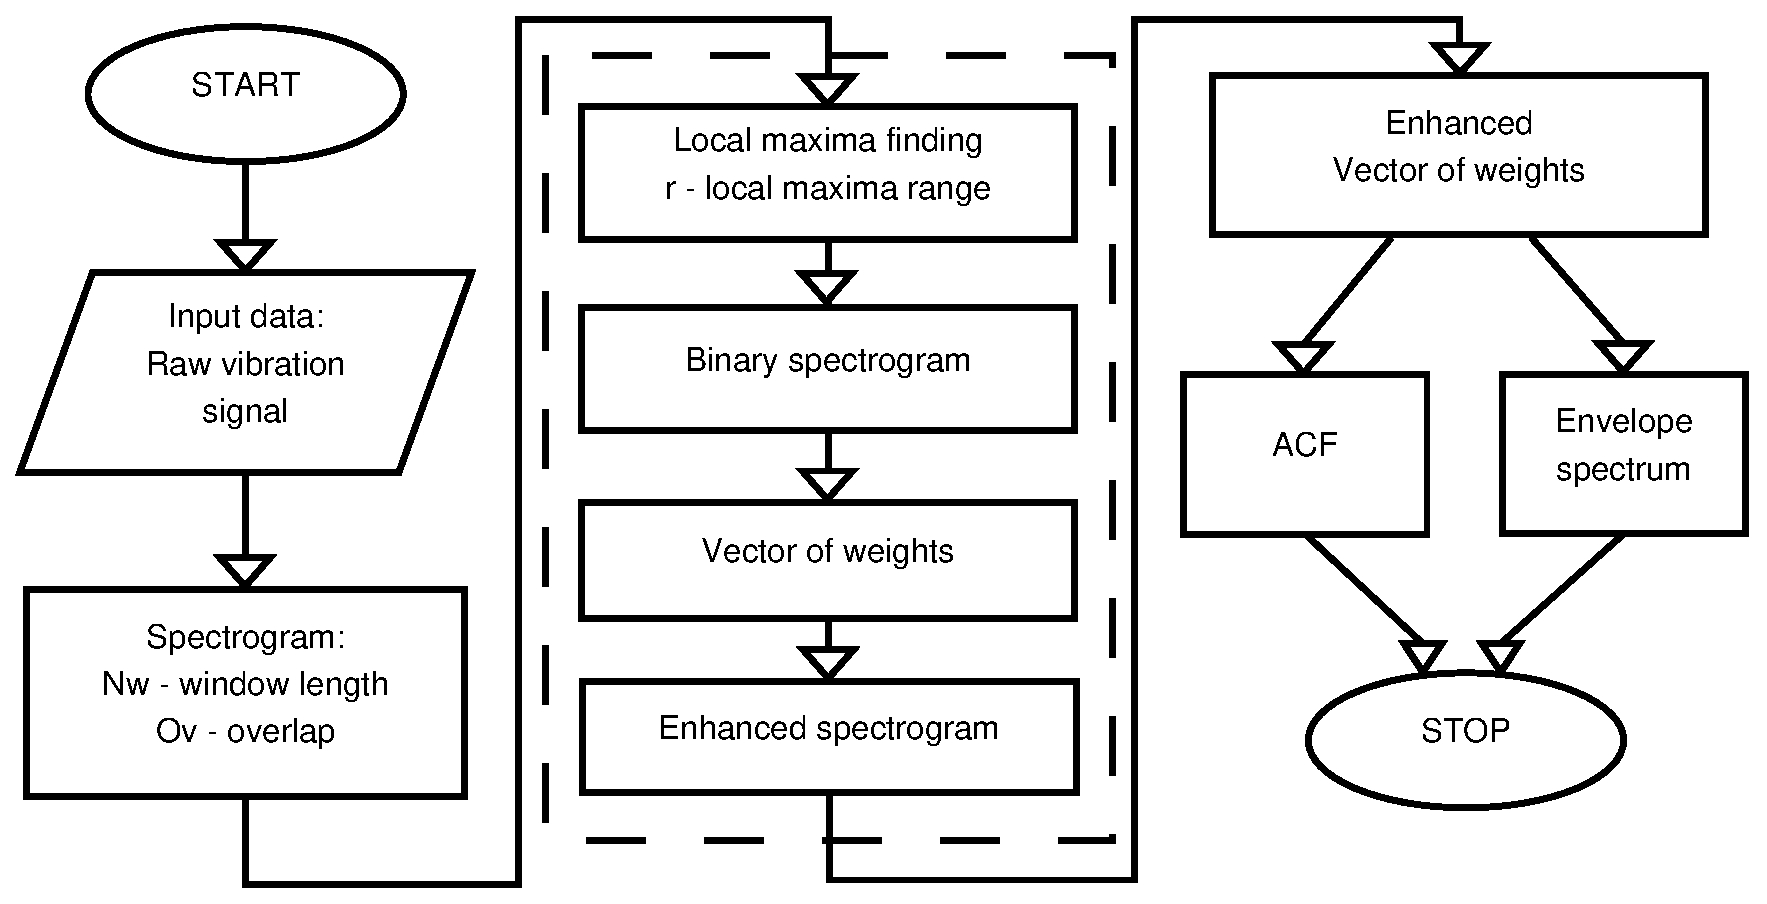
\includegraphics[width=0.7\textwidth]{fig01diagram.eps}
\caption{Diagram of time-frequency map enhancement procedure.}\label{fig01}
\end{center}
\end{figure}
\section{Simulated data analysis}\label{simulated}
To accurately illustrate the whole methodology  we analyze simulated signals that  represent acceleration of vibrations of both healthy and damaged bearing operating under industrial conditions where vibrations of a gearbox located nearby strongly contaminates the informative signal, i.e. the signal related to local damage. The raw signal is composed of deterministic components, i.e. high-energy sine waves related to vibrations of the gearbox and noise which in the case of damage is amplitude modulated with a frequency of $13$~[Hz] (fault frequency).
\begin{figure}[!ht]
\begin{center}
\includegraphics[width=0.7\textwidth]{fig02simFer-raw_signal_timeseries_g.eps}
\includegraphics[width=0.7\textwidth]{fig03simFer-raw_signal_timeseries.eps}
\caption{Time series of raw simulated data (first $0.25$ [s]), healthy (top panel) and faulty (bottom panel) bearing. Note three marked time points with barely visible disturbances.}\label{fig02}
\includegraphics[width=0.3\textwidth]{fig04simFer-raw_signal_spectrogram_g-ov-0.eps}
\includegraphics[width=0.3\textwidth]{fig05simFer-raw_signal_spectrogram_g-ov-0.95.eps}\\
\includegraphics[width=0.3\textwidth]{fig06simFer-raw_signal_spectrogram-ov-0.eps}
\includegraphics[width=0.3\textwidth]{fig07simFer-raw_signal_spectrogram-ov-0.95.eps}
\caption{Time-frequency representations (spectrograms) of the signals, healthy (top panels) and faulty (bottom panels) bearing, $95\%$ overlap case (right panels) and non-overlapping case (left panels).}
\label{fig03}
\includegraphics[width=0.33\textwidth]{fig08simFer-raw_signal_spectrogram_binary_g-ov-0.eps}
\includegraphics[width=0.33\textwidth]{fig09simFer-raw_signal_spectrogram_binary_g-ov-0.95.eps}\\
\includegraphics[width=0.33\textwidth]{fig10simFer-raw_signal_spectrogram_binary-ov-0.eps}
\includegraphics[width=0.33\textwidth]{fig11simFer-raw_signal_spectrogram_binary-ov-0.95.eps}
\caption{Binary spectrograms of the signals, healthy (top panels) and faulty (bottom panels) bearing, $95\%$ overlap case (right panels) and non-overlapping case (left panels).}\label{fig04}
\end{center}
\end{figure}
Length of both signals is $2.5$ [s], sampling frequency is $20000 $~[Hz]. The noise (amplitude modulated or not) is filtered at frequency range 3000-5000 Hz to imitate resonance effects. The signals are presented in Fig.~\ref{fig02} (time series) and Fig.~\ref{fig03} (spectrograms). For time-frequency representation a Kaiser window of length $230$ was used and FFT was calculated at $512$ points. In the overlapping case $95\%$ of segments overlaps, i.e. $219$ samples. Thus, non-overlapping case consists of $87$ spectra per second and overlapping case -- $1659$ spectra per second. It can be seen that energy of deterministic components is much higher than energy of the signal related to damage, thus the latter is barely-visible in time series plot.\\
Fig.~\ref{fig04} presents binary spectrograms in all cases, including data representing healthy and faulty bearing and both cases of overlapping. Here a theoretical ranges of local maxima were used, $r_0 =5$ and $r_{95\%} =113$. The case of healthy bearing plots looks totally random despite different content of each band that can be seen in Fig.~\ref{fig03}. In the damaged bearing case we obtain some wide-band lines related to local damage, but there is still a large amount of local maxima that do not follow any of them.
Applying formula (\ref{row4}) enhanced spectrograms are obtained (Fig.~\ref{fig06}).\\
\begin{figure}[!ht]
\begin{center}
\includegraphics[width=0.30\textwidth]{fig12simFer-wektor_wag1_timeseries_g-ov-0.eps}\includegraphics[width=0.30\textwidth]{fig13simFer-wektor_wag1_timeseries_g-ov-0.95.eps}\\
\includegraphics[width=0.30\textwidth]{fig14simFer-wektor_wag1_timeseries-ov-0.eps}
\includegraphics[width=0.30\textwidth]{fig15simFer-wektor_wag1_timeseries-ov-0.95.eps}
\caption{Vectors of weights of the signals, healthy (top panels) and faulty (bottom panels) bearing, $95\%$ overlap case (right panels) and non-overlapping case (left panels).}\label{fig05}
\includegraphics[width=0.33\textwidth]{fig16simFer-raw_signal_spectrogram_enh_g-ov-0.eps}
\includegraphics[width=0.33\textwidth]{fig17simFer-raw_signal_spectrogram_enh_g-ov-0.95.eps}\\
\includegraphics[width=0.33\textwidth]{fig18simFer-raw_signal_spectrogram_enh-ov-0.eps}
\includegraphics[width=0.33\textwidth]{fig19simFer-raw_signal_spectrogram_enh-ov-0.95.eps}
\caption{Enhanced spectrograms of the signals, healthy (top panels) and faulty (bottom panels) bearing, $95\%$ overlap case (right panels) and non-overlapping case (left panels).}\label{fig06}
\includegraphics[width=0.30\textwidth]{fig20simFer-wektor_wag_timeseries_g-ov-0.eps}
\includegraphics[width=0.30\textwidth]{fig21simFer-wektor_wag_timeseries_g-ov-0.95.eps}\\
\includegraphics[width=0.30\textwidth]{fig22simFer-wektor_wag_timeseries-ov-0.eps}
\includegraphics[width=0.30\textwidth]{fig23simFer-wektor_wag_timeseries-ov-0.95.eps}
\caption{Enhanced vectors of weights., healthy (top panels) and faulty (bottom panels) bearing, $95\%$ overlap case (right panels) and non-overlapping case (left panels).}\label{fig07}
\end{center}
\end{figure}
Basically, we multiply the vector of weights (Fig.~\ref{fig05}) by the binary spectrogram (Fig.~\ref{fig04}) .They share positive behavior of binary ones, because top panels in Fig.~\ref{fig06} still look randomly and bottom ones have clearly visible lines related to local damage. The biggest advantage of the local maxima method can be seen at non-informative frequency bands. Local maxima that do not follow any of wide-band excitations are reduced. In the overlapping case these local maxima almost completely disappeared. In this way, the informative frequency band is clearly visible.\\
After we have enhanced spectrograms in all of $4$ cases analyzed here, one can estimate the frequency of cyclic disturbances in time domain related to contact of rolling bearing elements with the local damage. Recall that the fault frequency is $13$~[Hz]. We have introduced enhanced vector of weights as an revised indicator of local maxima occurrence in time domain. Fig.~\ref{fig07} presents how the enhanced vectors of weights exhibit cyclic disturbances. Thus, we can use methods discussed in Sec.~\ref{methodology}.\\
\begin{figure}[ht]
\begin{center}
\includegraphics[width=0.38\textwidth]{fig24simFer-wektor_wag_envelope_g-ov-0.eps}
\includegraphics[width=0.38\textwidth]{fig25simFer-wektor_wag_envelope_g-ov-0.95.eps}\\
\includegraphics[width=0.38\textwidth]{fig26simFer-wektor_wag_envelope-ov-0.eps}
\includegraphics[width=0.38\textwidth]{fig27simFer-wektor_wag_envelope-ov-0.95.eps}
\caption{Envelope spectra of vectors of weights, healthy (top panels) and faulty (bottom panels) bearing, $95\%$ overlap case (right panels) and non-overlapping case (left panels). Red dashed lines denote fault frequency and its harmonics.}\label{fig08}
\includegraphics[width=0.38\textwidth]{fig28simFer-wektor_wag_acf_g-ov-0.eps}
\includegraphics[width=0.38\textwidth]{fig29simFer-wektor_wag_acf_g-ov-0.95.eps}\\
\includegraphics[width=0.38\textwidth]{fig30simFer-wektor_wag_acf-ov-0.eps}
\includegraphics[width=0.38\textwidth]{fig31simFer-wektor_wag_acf-ov-0.95.eps}
\caption{Sample autocorrelation functions, healthy (top panels) and faulty (bottom panels) bearing, $95\%$ overlap case (right panels) and non-overlapping case (left panels).}\label{fig09}
\end{center}
\end{figure}
Envelope spectra of vectors presented in Fig.~\ref{fig07} are shown in Fig.~\ref{fig08}. In the non-overlapping case resolution of data is too small to clearly recognize the fault frequency. There are few similar peaks in the bottom left panel, but only two of them are related to the expected frequencies. Thus, estimation cannot provide satisfactory results. High overlap of segments in STFT results in much better resolution of data and envelope spectra analysis of the enhanced vector of weights gives clear information about fault frequency. Set of decreasing harmonics indicate impulsive character of noise modulation.\\
Since envelope spectra give unsatisfactory results in the non-overlapping case we analyze the sample autocorrelation function. In the healthy bearing case almost all of autocorrelations are inside the $95\%$ confidence interval (Fig.~\ref{fig09}, top left panel). In the opposite case (Fig.~\ref{fig09}, bottom left panel) there are few lags at which the sample ACF significantly exceeds the confidence interval. The expected fault frequency is $13$~[Hz], so time interval between pulses is a multiple of about $0.0769$ [s] ($\frac{1}{ff}$). Recall that lag of $1$ sample stands for $0.0115$ [s], so lag of $7$ samples stands for $0.0805$ [s] and $12.42$~[Hz]. One can observe that high values of autocorrelation at lags of $13, 20, 27, 40$ and $47$ samples are related to multiplies of the expected time interval between pulses.\\
The sample ACF leads to useful results even in the case of high-overlapping windows in STFT. Here, $1$ lag equals to $0.0006$ [s], so the highest ACF should be manifested at lags of $128, 256, 385, 513, 641, 769$ and $897$ samples. Just a few high ACF values at first lags (Fig.~\ref{fig09}, right panels) indicates a short in time dependency and might be associated with high overlap.
\section{Machine and experiment description}\label{experiment}
In this section, results of an application of proposed technique to real machines operating in mining industry will be discussed. Mining machines seem to be a special class of machines with complex structure, high-power, time-varying load, etc.
\begin{figure}[!ht]
\begin{center}
\includegraphics[width=0.8\textwidth]{fig32przenosnik_szkic.eps}
\caption{a) Simplified diagram of a belt conveyor, b) location of monitored bearings.}\label{fig1R}
\end{center}
\end{figure}
\begin{figure}[!ht]
\begin{center}
\includegraphics[width=0.8\textwidth]{fig33przenosnik_fotki.eps}
\caption{A general view on belt conveyor driving stations: a) machine with drive pulley damage, b) machine with tension pulley damage.}\label{fig2R}
\end{center}
\end{figure}
In this paper, we will concentrate on belt conveyor system, widely used for continuous transport of bulk materials (coal, overburden, copper ore, etc) in both opencast and underground mines. Depends on the design (required power for driving of belt conveyor), belt conveyor driving station might consist of one up to four drive units with $630$ or $1000$ [kW] power each. Briefly, the design of belt conveyor is presented in Fig.~\ref{fig1R}.  From diagnostic point of view there are several critical elements in belt conveyor: drive unit (electric motor, coupling, gearbox and drive pulley), non-drive pulley, belt and idlers. In this paper only bearings used in both: drive and non-drive pulleys are investigated.\\
Photographs of investigated machines working in the mining company are presented in Fig.~\ref{fig2R}. In case discussed here, two drive units are used (note blue housing of electric motors in Fig~\ref{fig2R}a and b). There are some differences in design between presented systems, moreover, as it will be shown two different problems appeared in pulleys. First, a system presented in Fig.~\ref{fig2R}a with drive pulley bearing problem will be discussed, second, system from Fig.~\ref{fig2R}b, with tension pulley bearing will be investigated.\\
\textbf{Case A}. The task is defined as condition monitoring of bearings used in drive pulleys. In Fig.~\ref{fig33}a the scheme of the drive unit for a belt conveyor is shown. The drive unit consists of an electric motor, a coupling and two stage gearbox, that are connected with a pulley.
\begin{figure}[!ht]
\begin{center}
\includegraphics[width=0.8\textwidth]{fig34beben_abcd.eps}
\caption{Diagnosed object A: a) Scheme, b) Pulley with bearing housing mounted on shaft, c) View on joint of output shaft in gearbox with pulley, d) View on sensor location on pulley.
}\label{fig33}
\end{center}
\end{figure}
The pulley (Fig.~\ref{fig33}b) consists of a shaft, two bearings and the coating covered by rubber (to increase friction between the pulley coating and the belt). Often between the gearbox and the pulley a rigid coupling is used (see Fig.~\ref{fig33}c). The location of accelerometer is shown in Fig.~\ref{fig33}d: the sensor has been mounted using screw, in horizontal direction. It is important to notice that level of vibration generated by drive unit elements (mainly gearbox) is much higher than vibration produced by pulley. In other words, practically, bearings signature is hidden in mixture of gearbox and pulley vibrations.\\
\textbf{Case B}. Second case is related to condition monitoring of bearings used in tension pulley, presented in Fig~\ref{fig44}a. It is not equipped with drive unit. Purpose of this pulley is to assure appropriate tension inside the belt, it is a part of mechanical automatic control system presented in Fig~\ref{fig44}b. Despite the fact that level of external noise is much less, and impact coming from damaged bearing are visible, some extra processing is required.
\begin{figure}[!ht]
\begin{center}
\includegraphics[width=0.8\textwidth]{fig35beben_fotki.eps}
\caption{A general view of tension pulley and its location in tensioning system in belt conveyor}
\label{fig44}
\end{center}
\end{figure}
\subsection{Experiments. Basic data}
In both considered cases several signal acquisition sessions have been performed. In Case A commercial diagnostic system installed on the machine and operating in online mode was used to acquire data for offline processing. In Case B, portable data acquisition system (notebook, NI DAq) was used. Location of the sensors are presented in Fig.~\ref{fig33}d (Case A) and in Fig.~\ref{fig55} (Case B).\\
\begin{figure}[ht]
\begin{center}
\includegraphics[width=0.65\textwidth]{fig36czujnik.eps}
\caption{Accelerometer locations during experiments.}
\label{fig55}
\end{center}
\end{figure}
\begin{table}[ht]
\caption{Theoretical frequencies for both machines.}
\centering
\begin{tabular}[]{|r|r|r|}\hline%\hline
Frequency	&Drive pulley	&Tension Pulley\\ \hline 
$f_{FTF}$& 	$0.51 Hz$&	$0.6$\\\hline
$f_{BSF}$&	$4.45 Hz$&	$3.53$\\ \hline
$f_{BFF}$& $8.90 Hz$&$	7.07$\\\hline
$f_{BPFO}$&	$12.34 Hz$&	$8.11$\\\hline
$f_{BPFI}$& $16.06 Hz$&	1$0.8$\\\hline
$$&sampling frequency&sampling frequency\\
 $$&$f_s = 19200 Hz$&$f_s = 16384 Hz$\\
$$& duration & duration\\
$$&$T = 2.5 s$&$T = 40 s$\\\hline%\hline.
\end{tabular}\label{tab1}
\end{table}
Before experiments some basic characteristics were estimated. Based on the bearing geometry and the shaft's rotational speed, the characteristic defect frequencies of rolling bearings were calculated, see Table~\ref{tab1}. Mentioned frequencies stand for: $f_{FTF}$ - fundamental train frequency, $f_{BSF}$ - ball spin frequency, $f_{BFF}$ - ball fault frequency, $f_{BPFO}$ - ball passing frequency outer race, $f_{BPFI}$ - ball passing frequency inner race.\\
For Case A two vibration signals generated by the drive unit, including vibration data of undamaged and damaged bearings, are available. Due to rigid connection between gearbox and pulley, a serious participation of gearbox vibration in acquired vibration signal has been noticed. Energy of signal components related to gear meshing frequency completely masks the signal of interest - the signal from the rolling bearing. For Case B vibration signals acquired from faulty bearings are available (no healthy condition reference). For both cases machine was loaded, i.e. bulk material on the belt was present.
\section{Real data processing results}\label{real}
\textbf{Case A}. In this section a real dataset  described in the previous section is analyzed.
\begin{figure}[!ht]
\begin{center}
\includegraphics[width=0.9\textwidth]{fig38real_Fer-raw_signal_timeseries_g.eps}
\includegraphics[width=0.9\textwidth]{fig39real_Fer-raw_signal_timeseries.eps}
\caption{Time series of raw real data, healthy (top panel) and faulty (bottom panel) bearing.}
\label{fig10}
\includegraphics[width=0.4\textwidth]{fig40real_Fer-raw_signal_spectrogram_g-ov-0.eps}
\includegraphics[width=0.4\textwidth]{fig41real_Fer-raw_signal_spectrogram_g-ov-0.95.eps}\\
\includegraphics[width=0.4\textwidth]{fig42real_Fer-raw_signal_spectrogram-ov-0.eps}
\includegraphics[width=0.4\textwidth]{fig43real_Fer-raw_signal_spectrogram-ov-0.95.eps}
\caption{Time-frequency representations (spectrograms) of the signals, healthy (top panels) and faulty (bottom panels) bearing, $95\%$ overlap case (right panels) and non-overlapping case (left panels).}
\label{fig11}
\end{center}
\end{figure}
Fig.~\ref{fig10} and Fig.~\ref{fig11} presents time series and spectrograms, respectively, of both (healthy and faulty) signals. Spectrograms were calculated with and without overlap. The Kaiser window of lenght $200$ was used. In this case  $95\%$ overlap case stands for $190$ samples. Fast Fourier transform is calculated in $512$ points. These parameters result in $96$ and $1912$ spectra in non- and $95\%$ overlapping case, respectively.\\
\begin{figure}[!ht]
\begin{center}
\includegraphics[width=0.38\textwidth]{fig44real_Fer-raw_signal_spectrogram_binary_g-ov-0.eps}
\includegraphics[width=0.38\textwidth]{fig45real_Fer-raw_signal_spectrogram_binary_g-ov-0.95.eps}\\
\includegraphics[width=0.38\textwidth]{fig46real_Fer-raw_signal_spectrogram_binary-ov-0.eps}
\includegraphics[width=0.38\textwidth]{fig47real_Fer-raw_signal_spectrogram_binary-ov-0.95.eps}
\caption{Binary spectrograms of the signals, healthy (top panels) and faulty (bottom panels) bearing, $95\%$ overlap case (right panels) and non-overlapping case (left panels).}
\label{fig12}
\includegraphics[width=0.38\textwidth]{fig48real_Fer-raw_signal_spectrogram_enh_g-ov-0.eps}
\includegraphics[width=0.38\textwidth]{fig49real_Fer-raw_signal_spectrogram_enh_g-ov-0.95.eps}\\
\includegraphics[width=0.38\textwidth]{fig50real_Fer-raw_signal_spectrogram_enh-ov-0.eps}
\includegraphics[width=0.38\textwidth]{fig51real_Fer-raw_signal_spectrogram_enh-ov-0.95.eps}
\caption{Enhanced spectrograms of the signals, healthy (top panels) and faulty (bottom panels) bearing, $95\%$ overlap case (right panels) and non-overlapping case (left panels).}
\label{fig13}
\end{center}
\end{figure}
Both signals contain a high-energy contamination, but its frequency band is relatively narrow. The informative frequency band, i.e. band, where wide-band excitations occurs, approximately starts at $1000$~[Hz] and ends at $6000$~[Hz], but there are few pulses whose bandwidth is wider.\\
The ranges of local maxima we have chosen here are equal to the theoretical ones, $r_0 =6$ and $r_{95\%} =131$. Due to local character of damage the time of impulse relaxation is quite short and shortening the ranges is not necessary. Binary spectrograms (Fig.~\ref{fig12}) for healthy bearing real data look randomly and (as in Sec.~\ref{simulated}) none of frequency bands can be singled out. In the faulty bearing case almost continuous wide lines can be seen. They are a little bit longer than those presented in Fig.~\ref{fig11}.\\
Enhanced spectrograms clearly present length of the informative frequency band with non-informative components removed (Fig.~\ref{fig13}). While enhanced versions of time-frequency maps in healthy bearing case are still random, in the faulty case one can see almost only cyclically occurring wide lines.\\
\begin{figure}[!ht]
\begin{center}
\includegraphics[width=0.36\textwidth]{fig52real_Fer-wektor_wag_timeseries_g-ov-0.eps}
\includegraphics[width=0.36\textwidth]{fig53real_Fer-wektor_wag_timeseries_g-ov-0.95.eps}\\
\includegraphics[width=0.36\textwidth]{fig54real_Fer-wektor_wag_timeseries-ov-0.eps}
\includegraphics[width=0.36\textwidth]{fig55real_Fer-wektor_wag_timeseries-ov-0.95.eps}
\caption{Enhanced vectors of weights, healthy (top panels) and faulty (bottom panels) bearing, $95\%$ overlap case (right panels) and non-overlapping case (left panels).}
\label{fig14}
\includegraphics[width=0.36\textwidth]{fig56real_Fer-wektor_wag_envelope_g-ov-0.eps}
\includegraphics[width=0.36\textwidth]{fig57real_Fer-wektor_wag_envelope_g-ov-0.95.eps}\\
\includegraphics[width=0.36\textwidth]{fig58real_Fer-wektor_wag_envelope-ov-0.eps}
\includegraphics[width=0.36\textwidth]{fig59real_Fer-wektor_wag_envelope-ov-0.95.eps}
\caption{Envelope spectra of vectors of weights. Healthy (top panels) and faulty (bottom panels) bearing, $95\%$ overlap case (right panels) and non-overlapping case (left panels). Red dashed lines denote fault frequency and its harmonics.}
\label{fig15}
\includegraphics[width=0.36\textwidth]{fig60real_Fer-wektor_wag_acf_g-ov-0.eps}
\includegraphics[width=0.36\textwidth]{fig61real_Fer-wektor_wag_acf_g-ov-0.95.eps}\\
\includegraphics[width=0.36\textwidth]{fig62real_Fer-wektor_wag_acf-ov-0.eps}
\includegraphics[width=0.36\textwidth]{fig63real_Fer-wektor_wag_acf-ov-0.95.eps}
\caption{Sample autocorrelation functions, Healthy (top panels) and faulty (bottom panels) bearing, $95\%$ overlap case (right panels) and non-overlapping case (left panels).}
\label{fig16}
\end{center}
\end{figure}
Fig.~\ref{fig14} shows enhanced vectors of weights -- result of application of formula (\ref{row4}). Their envelopes spectra are presented in Fig.~\ref{fig15}. As it can be seen, higher resolution obtained by using $95\%$ overlap enabled to estimate the fault frequency even using envelope spectrum. In this case, the estimated fault frequency is $12.69$~[Hz] and is related to the frequency characteristic for outer race local damage.\\
As it was mentioned, one of the  method that can be used to estimate the fault frequency is the sample ACF. Due to industrial origin of the data only few values of sample ACF exceeds the $95\%$ confidence interval in the faulty bearing case (Fig.~\ref{fig16}). Time interval between observations is $0.0104$ [s] and $0.00052$ [s] in non-overlapping and $95\%$ overlapping case, respectively. Thus, in the first case fault frequency of $12.69$~[Hz] stands for about $7.565$ "samples", so high value of the ACF at lag $7, 8$ and $15$ clearly confirms the fault frequency close to $12.8$~[Hz]. In the second case the ACF should be significantly higher at lags that are multiplies of $151$ samples.\\
\textbf{Case B}. To complete analysis we present how the local maxima method deals with real dataset described in the previous section in Case B.  Fig.~\ref{fig17} and Fig.~\ref{fig18} presents time series and spectrograms, respectively.\\
\begin{figure}[ht]
\begin{center}
\includegraphics[width=0.9\textwidth]{fig64real-raw_signal_timeseries.eps}
\caption{Time series of raw real data.}
\label{fig17}
\includegraphics[width=0.45\textwidth]{fig65real-raw_signal_spectrogram-ov-0.eps}
\includegraphics[width=0.45\textwidth]{fig66real-raw_signal_spectrogram-ov-0.95.eps}
\caption{Time-frequency representations (spectrograms) of the signals, $95\%$ overlap case (right panel) and non-overlapping case (left panel).}
\label{fig18}
\includegraphics[width=0.43\textwidth]{fig67real-raw_signal_spectrogram_binary-ov-0.eps}
\includegraphics[width=0.43\textwidth]{fig68real-raw_signal_spectrogram_binary-ov-0.95.eps}
\caption{Binary spectrograms of the signals, $95\%$ overlap case (right panel) and non-overlapping case (left panel).}\label{fig19}
\end{center}
\end{figure}
Here a Kaiser window of length $1000$ samples is used with $95\%$ overlap and without it obtaining $16$ and $327$ spectra per second. Number of FFT points used for spectrograms is $1024$. Few disturbances with low frequency are visible, but the informative frequency band is much shorter than in the case analyzed in Case A.\\
\begin{figure}[!ht]
\begin{center}
\includegraphics[width=0.43\textwidth]{fig69real-raw_signal_spectrogram_enh-ov-0.eps}
\includegraphics[width=0.43\textwidth]{fig70real-raw_signal_spectrogram_enh-ov-0.95.eps}\caption{Enhanced spectrograms of the signals, $95\%$ overlap case (right panel) and non-overlapping case (left panel).}\label{fig20}
\includegraphics[width=0.43\textwidth]{fig71real-wektor_wag_timeseries-ov-0.eps}
\includegraphics[width=0.43\textwidth]{fig72real-wektor_wag_timeseries-ov-0.95.eps}\caption{Enhanced vectors of weights, $95\%$ overlap case (right panel) and non-overlapping case (left panel).}\label{fig21}
\includegraphics[width=0.43\textwidth]{fig73real-wektor_wag_envelope-ov-0.eps}
\includegraphics[width=0.43\textwidth]{fig74real-wektor_wag_envelope-ov-0.95.eps}
\caption{Envelope spectra of vectors of weights, $95\%$ overlap case (right panel) and non-overlapping case (left panel). Red dashed lines denote fault frequency and its harmonics.}\label{fig222}
\includegraphics[width=0.4\textwidth]{fig75real-wektor_wag_acf-ov-0.eps}
\includegraphics[width=0.4\textwidth]{fig76real-wektor_wag_acf-ov-0.95.eps}
\caption{Sample autocorrelation functions, $95\%$ overlap case (right panel) and non-overlapping case (left panel).}\label{fig23}
\end{center}
\end{figure}
Binary spectrograms (Fig.~\ref{fig19}) in both cases are very noisy and lines related to wide-band excitations are barely visible. After applying (\ref{row3}) the enhanced spectrograms look much clearer (Fig.~\ref{fig20}). In the case of $95\%$ overlap non-significant local maxima are almost completely removed at the expense of visibility of desired results. Recall that in this dataset the expected fault frequency is very low ($0.6$~[Hz] - cage damage) comparing to the fault frequency in data analyzed in previous sections ($13$~[Hz]) because of different types of damage. It is worth mentioning that great resolution in time is presented even in non-overlapping case, so high overlapping is not necessary here. Nevertheless, it causes problems only in presentation of final enhanced spectrogram -- wide-band lines are still visible, but there are thin, so they seem to be weaker than in non-overlapping case.\\
Fig.~\ref{fig21},~\ref{fig222} and~\ref{fig23} present enhanced vectors of weights, envelope spectra and sample ACF of them, respectively. Recall that the expected fault frequency is $0.6$~[Hz]. From Fig.~\ref{fig222} it can be found that the fault frequency is $0.73$ Hz. The difference between the expected and estimated frequency might be caused by different that assumed operating conditions. This frequency and its harmonics are much better visible when the STFT segments highly overlap each other. When the segments do not overlap there are some significant peaks in envelope spectrum, but their values are lower than first two harmonics of fault frequency.\\
Due to different kind of damage than in previous case shape of the sample autocorrelation functions is specific, but it  is still a good estimator of fault frequency. Since one sample of enhanced vector of weights equals to $0.061$ [s] while STFT do not overlap and $0.00305$ [s] when they do ($95\%$ overlap) one can expect higher value of autocorrelation at lag that are multiplies of $11$ and $224$ samples, respectively.
\section{Discussion}\label{discussion}
Classical methods of local damage detection might be divided into groups using several features of the signal which occurs in case of local damage in a rotating machine. Among the features one can distinguish impulsiveness, cyclicity of disturbances, random character of the informative signal and shape of the impulse occurred during contact with a damaged surface. Here we briefly recall properties of classical methods and compare them to the local maxima method.\\
Prominent examples of methods that exploit impulsive character of the signal related to the fault are the methods based on kurtosis (e.g. spectral kurtosis, the kurtogram, minimum entropy deconvolution)~\cite{bib4,bib5,bib6}. Kurtosis is a statistical measure that quantifies dispersion of a process. If the signal contains time points where amplitude is significantly higher than elsewhere then kurtosis gains. Even a single impulse increases this statistical characteristic, so it is sensitive to outliers not related to damage. Such situation might occur during data acquisition in industrial conditions. This uncertainty might be minimized using other measures of impulsiveness that are less sensitive to single impacts and still sensitive to impulses related to the local damage. Spectral kurtosis relies on quantifying kurtosis of narrow frequency bins. Then a filter is designed that increases influence of bands with high kurtosis and decreases others. The methodology exploits the short time Fourier transform and strongly depends on the STFT window. The kurtogram is an attempt to present dependency between STFT window and spectral kurtosis. Calculating SK for every window length is computationally intensive and differences between windows of similar length are not significant. The fast kurtogram calculates SK for particular window lengths only, i.e. windows obtained by e.g. binary or trinary partition of the whole frequency spectrum. Minimum entropy deconvolution, called also "maximum kurtosis deconvolution" designs an inverse filter that maximizes kurtosis of the output. The inverse filter output is related to the input of the system. Thus, original impulses are raised which results in the raw signal enhancement.\\
The local maxima also exploits impulsiveness  of the signal related to damage and its spectral representation. Spectrum of an impulse signal contains wideband excitation, so spectrogram contains series of local, equally spaced wideband excitations, i.e. energy at the time of impulse is higher than in some time before and after the impulse. Thus, it might be said that a local maximum occurs. Significance of all of local maxima in the spectrogram is quantified in subsequent steps of the local maxima method.\\
The next group of classical local damage detection methods contains methods based on random character of impacts~\cite{bib19,bib20,bib26,bib27,ANCZhou,SANC1,SANC2,SANC3, SANC4,TSA1,DRS}. In spite of deterministic, discrete frequency components contribution of local damage in the vibration signal is assumed to be random. One of the most fundamental methods is linear prediction - a procedure which predicts the signal as a weighted sum of past values. The number of past values and weights used for prediction might be determined using several criteria, e.g. Akaike information criterion (AIC), Bayesian information criterion (BIC). Unpredictable part of the signal includes random signal with deterministic components removed. There is also a method that engages an additional, reference signal - adaptive noise cancellation (ANC). It is a procedure that separates two uncorrelated components which form the signal by using an additional signal that represents only one of the parts. The additional signal must be related to its counterpart only by a linear transfer function. Then the ANC adaptively finds the transfer function and separates components of the raw signal. This method relies on the ability of the reference signal acquisition, thus it cannot be applied to local damage detection in cases where it is impossible to acquire the reference signal. In this case it is impossible to acquire a signal that is uncorrelated with the signal related to local damage. To overcome this problem one can use self-adaptive noise cancellation (SANC). The reference signal is obtained not by additional data acquisition but by delaying the primary signal. If the delay is appropriate, than the adaptive filter will not identify correlation between delayed primary signal and the random part. Unfortunately, estimation procedure of parameters used in this method might be divergent. In the literature it is said that discrete/random separation gives similar results without such risk. In a case of small speed variations or if they might be suppressed by pre-processing methods such as order-tracking one can predict the raw signal from its delayed version by using a technique in frequency domain called discrete-random separation (DRS). The technique is based on FFT, thus computation time is much lower than in SANC while results of both method are comparable. There are also papers in which a similar problem is analyzed, i.e. local damage detection in bearings operating in a belt conveyor driving system that works in a mining company and adaptive filtering is being used. One of them presents a technique based on adaptive filter designing which uses reflection coefficients in adaptive Schur filter~\cite{bib19}. The second one incorporates Normalised Least Square Mean (NLSM) adaptive filter for weak impulsive signal recovery. Sometimes DRS might remove narrow band noise peaks that does not follow any deterministic components. In such case time synchronous averaging (TSA) might be used in order to prevent removal of relevant information. This advantage of TSA is paid with a need for specifying sets of harmonics for each discrete frequency separately. Contrary, the local maxima method needs no information about deterministic frequencies to minimize their influence on further processing. These signal components are removed by the method itself, because frequency band of a discrete frequency is narrow in opposite to frequency band of an impulse, which is said to be wide. Thus, local maxima occurred in frequency bins that does not follow any wideband excitation have insignificant influence on the vector of weights (and its enhanced version as well). The method also does not distinguish between high- and low- energy components if only they share similar behavior of local maxima occurrence (random or cyclic). As a result, high energy components are not blindly removed regardless of whether they represent uncertain noise or informative residual signal. The key feature of a frequency bin is that it contains local maxima occurred at the same time in other frequency bins or they are random. Furthermore, there is no need for additional signal to benefit from advantages of the local maxima method.\\
The most promising and powerful approach is focused on searching for hidden (fault induced) periodicity of random signals by cyclostationary signal modeling and analysis. Searching of two dimensional correlation function and its spectral representation provide bi-frequency map (carrier frequency versus modulating frequency) that clearly indicates whether  modulation exist and what is the frequency related to damage. Deep study provided by Antoni~\cite{CYCLAntoni} and further extension provided by Urbanek et al.~\cite{MID} (MID - modulation intensity density) shows that such technique is able to extract information. Antoni and Randall proved that there is a link between integrated SCD and envelope spectrum. The enhanced spectrogram might be treated as a two-dimensional representation of cyclic impulsive disturbances. Thus, the vector of weights is a kind of envelope that quantifies cyclic disturbances of an impulsive character in one dimension.\\
The last classical methods we discuss is a wavelet approach~\cite{WaveletReview}. In general, it is based on shape of an impulse occurred during contact of a damaged surface. If the wavelet is similar to the impulse than they are correlated. Thus, time points of the raw signal with high correlation are indicated as moments of contact with the damaged surface. The problem in this approach is to find the proper wavelet that share shape with the impulse related to local damage. The advantage of this approach is its insensitivity to impulses of other shapes that might be not related to local damage. The local maxima method does not differentiate between different shapes of impulse until they form spectral lines of similar width on the spectrogram. If only an impulse not related to local damage occurs in the raw signal then the vector of weights contains it as well. If not, one can benefit from lack of need to determine shape of the wavelet.\\
Another interesting technique that is data driven, depends of the shape of the signal and decomposes (as wavelets) signal into set of IMFs functions is Empirical Mode Decomposition. Recent synthesis of this method might be find in review paper by Lei et al.~\cite{EMDLei}. The dataset analyzed in the present paper was also examined using EMD-based techniques. In~\cite{EMDZimroz} authors obtained similar results for the damaged bearing signal analyzed in Sec.~\ref{real} (Case A).\\
It should be said that instead of spectrogram other time-frequency representation with better time-frequency resolution might be used - see recent review of possible time-frequency representations~\cite{TFReview}. The proposed method (i.e. local maxima) should work even better in such a case.\\
It might be concluded that there are many available techniques that could be used for local damage detection. Some of them (SANC, EMD, wavelets\ldots) have been already applied for the same data as used in this paper and honestly it is hard to point out the best one - they provide similar (good) results. The method proposed in this paper is another technique that in our opinion is intuitive, simple and powerful.
\section{Conclusions}
In the paper a novel method of time-frequency map enhancement and further processing for feature extraction for local damage detection is proposed. The methodology was presented using spectrogram, however, it should be highlighted that the procedure might be applied to other time-frequency representation. Spectrogram enhancement is based on extraction of slice of spectrogram along time for each frequency bin, treating it as time series, and processing of each sub-signal for each frequency bin separately. Simple procedure is proposed to find local increase of amplitude that might correspond to impulsive disturbance related to shock caused by damage. Validation procedure of detected maxima is proposed. After local maxima detection and validation for each frequency bin, a new time-frequency map is created. It contains clear information that can be also easily aggregated to one-dimensional time series with cyclic impulses clearly visible. Original raw vibration signal contains strong non-informative contribution so detection of cyclic impulses related to damage is not possible. The advantage of the method is that after processing, high energy contributions with non-informative local maxima for some frequency bins have been - in some sense - neglected; sub-signals with cyclic disturbances are enhanced. It provides new time-frequency map with highlighted informative part. Finally, after agreegation 2D map to 1D time series, classic approach has been applied. Unfortunately, for spectrogram without overlapping, time resolution of the map is poor, so consequently aggregated time series will have poor resolution too. We propose to use sample ACF to detect periodicity in the signal, if classic envelope spectrum fails. Simulation as well as two case studies confirm efficiency of proposed approach.
\section*{References}
\begin{thebibliography}{00}
\bibitem{bib1}	Samuel, P.D., Pines, D.J., A review of vibration-based techniques for helicopter transmission diagnostics, Journal of Sound and Vibration 282(1-2) (2005) 475-508. 
\bibitem{bib2}	Randall, R.B., Antoni, J., Rolling element bearing diagnostics-A tutorial, Mechanical Systems and Signal Processing, 25(2) (2011)  485-520.
\bibitem{bib28} McFadden, P.D, Smith, J.D, Vibration monitoring of rolling element bearings by the high frequency resonance technique - a review, Tribology International 17(1) (1984) 3-10.
\bibitem{bib3}	Obuchowski, J., Wy{\l}oma{\'n}ska, A., Zimroz, R., The local maxima method for enhancement of time-frequency map, Advances in Condition Monitoring of Machinery in Non-Stationary Operations. In Dalpiaz, G.; et al (Eds.) Proceedings of the third International Conference Condition Monitoring of Machinery in Non-Stationary Operations CMMNO 2013, Series: Lecture Notes in Mechanical Engineering IX 2014,  pp. 325-334, Springer.
\bibitem{bib4}	Antoni, J., Randall, R.B., The spectral kurtosis: application to the vibratory surveillance and diagnostics of rotating machines, Mechanical Systems and Signal Processing 20(2) (2006) 308-331. 
\bibitem{bib5}	Antoni, J., Fast computation of the kurtogram for the detection of transient faults, Mechanical Systems and Signal Processing  21(1) (2007) 108-124.
\bibitem{bib6}	Barszcz, T., Jab{\l}o{\'n}ski, A.,  A novel method for the optimal band selection for vibration signal demodulation and comparison with the Kurtogram, Mechanical Systems and Signal Processing 25(1) (2011) 431-451.
\bibitem{bib7}	Obuchowski, J., Wylomanska, A., Zimroz, R., Stochastic modeling of time series with application to local damage detection in rotating machinery (2013) Key Engineering Materials, 569-570, 441-448.
\bibitem{bib14}	Urbanek, J., Barszcz, T., Antoni, J., Time-frequency approach to extraction of selected second-order cyclostationary vibration components for varying operational conditions, Measurement: Journal of the International Measurement Con-federation 46(4) (2013) 1454-1463.
\bibitem{bib15}	Urbanek, J., Barszcz, T., Zimroz, R., Antoni, J.,  Application of averaged instantaneous power spectrum for diagnostics of machinery operating under non-stationary operational conditions, Measurement: Journal of the International Measurement Confederation 45(7) (2012) 1782-1791.
%Filtering
\bibitem{bib16}	Lin, J., Zuo, M.,  Gearbox fault diagnosis using adaptive wavelet filter, Mechanical  Systems and Signal Processing 17(6) (2003) 1259-1269.
\bibitem{bib19}	Makowski, R., Zimroz, R., A procedure for weighted summation of the derivatives of reflection coefficients in adaptive Schur filter with application to fault detection in rolling element bearings, Mechanical Systems and Signal Processing 38(1) (2013) 65-77.
\bibitem{bib20}	Zimroz, R., Bartelmus, W., Application of adaptive filtering for weak impulsive signal recovery for bearings local damage detection in complex mining mechanical systems working under condition of varying load, Diffusion and Defect Data Pt.B: Solid State Phenomena 180 (2012) 250-257.
\bibitem{bib21}	Antoni, J., Randall, R.B., Differential diagnosis of gear and bearing faults, ASME Journal of Vibration and Acoustics, 124(2) (2002) 165-171.
\bibitem{bib22}	Barszcz, T., Decomposition of vibration signals into deterministic and nondeterministic components and its capabilities of fault detection and identification, International Journal of Applied Mathematics and Computer Science, 19(2) (2009) 327-335.
\bibitem{bib23}	Combet, F., Gelman, L., Optimal filtering of gear signals for early damage detection based on the spectral kurtosis, Mechanical Systems and Signal Processing 23(3) (2009) 652-668.
\bibitem{bib26}	Makowski, R.A., Zimroz, R., Adaptive bearings vibration modelling for diagnosis, Lecture Notes in Computer Science (including subseries Lecture Notes in Artificial Intelligence and Lecture Notes in Bioinformatics) 6943 LNAI (2011) 248-259.
\bibitem{bib27}	Makowski, R.A., Zimroz, R., New techniques of local damage detection in machinery based on stochastic modelling using adaptive Schur filter, Applied Acoustics 77 (2014) 130-137.
\bibitem{bib17}	Javorskyj, I., Le{\'s}kow, J., Kravets, I., Isayev, I., Gajecka, E., Linear filtration methods for statistical analysis of periodically correlated random processes - Part I: Coherent and component methods and their generalization, Signal Processing 92(7) (2012) 1559-1566.
\bibitem{bib18}	Javorskyj, I., Le{\'s}kow, J., Kravets, I., Isayev, I., Gajecka, E., Linear filtration methods for statistical analysis of periodically correlated random processes - Part II: Harmonic series representation, Signal Processing 91(11) (2011) 2506-2519.
\bibitem{bib8}	Safizadeh, M.S., Lakis A.A., Thomas M.,  Using short-time fourier transforms in machinery fault diagnosis, International Journal of Comadem 3(1) (2000) 5-16.
\bibitem{bib9}	Baydar, N., Ball, A., A comparative study of acoustic and vibration signals in detection of gear failures using Wigner-Ville distribution, Mechanical Systems and Signal Processing 15(6) (2011) 1091-1107.
\bibitem{bib10}	Lee, S.K., White, P., The L-Wigner Distribution and its use as a tool for condition monitoring, International Journal of Comadem 4(1) (2001) 5-11.
\bibitem{bib11}	Dalpiaz, G., Rivola, A., Rubini, R.,  Effectiveness and sensitivity of vibration processing techniques for local fault detection in gears,  Mechanical  Systems and Signal Processing 14(3) (2000) 387-412.
\bibitem{bib12}	Lee, S.K., White, P.R., Higher-order time-frequency analysis and its application to fault detection in rotating machinery,  Mechanical Systems and Signal Processing 11(4) (1997) 637-650.
\bibitem{bib13}	Peng, Z.K., Chu, F.L.,  Application of the wavelet transform in machine condition monitoring and fault diagnostics: a review with applications, Mechanical Systems and Signal Processing 18(2) (2004) 199-221.
\bibitem{HeManifold}	He, Q., Liu, Y., Long, Q., Wang, J., Time-frequency manifold as a signature for machine health diagnosis, IEEE Transactions on Instrumentation and Measurement 61(5) (2012) 1218-1230.
\bibitem{WangScale} Wang, J., He, Q., Kong, F., Automatic fault diagnosis of rotating machines by time-scale manifold ridge analysis, Mechanical Systems and Signal Processing 40(1) (2013) 237-256.
\bibitem{ANCZhou} Zhou, X., Shao, Y., Adaptive noise cancellation based on beehive pattern evolutionary digital filter, Mechanical Systems and Signal Processing 42(1-2) (2014) 225-235.
\bibitem{SANC1} Antoni, J., Randall, R.B., Optimisation of SANC for separating gear and bearing signals, in: Proceedings of the Comadem Conference, Manchester, September, (2001) 89-96.
\bibitem{SANC2} Ho, D., Randall, R.B., Optimization of bearing diagnostic techniques using simulated and actual bearing fault signals, Mechanical Systems and Signal Processing 14(5) (2000) 763-788.
\bibitem{SANC3} Antoni, J., Randall, R.B., Unsupervised noise cancellation for vibration signals: part I - evaluation of adaptive algorithms, Mechanical Systems and Signal Processing 18 (2004) 89-101.
\bibitem{SANC4} Antoni, J., Randall, R.B., Unsupervised noise cancellation for vibration signals: part II - a novel frequency-domain algorithm, Mechanical Systems and Signal Processing 18(1) (2004) 103-117.
\bibitem{TSA1} McFadden, P.D., A revised model for the extraction of periodic waveforms by time domain averaging, Mechanical Systems and Signal Processing, 1(1) (1987) 83-95.
\bibitem{DRS} Sawalhi, N., Randall, R.B., Localised fault diagnosis in rolling element bearings in gearboxes, in: Proceedings of the Fifth International Conference on Condition Monitoring and Machinery Failure Prevention Technologies (CM-MFPT), Edinburgh, (2008).
\bibitem{CYCLAntoni} Antoni, J., Cyclostationarity by examples, Mechanical Systems and Signal Processing, 23(4) (2009) 987-1036.
\bibitem{MID} Urbanek, J., Antoni, J., Barszcz, T., Detection of signal component modulations using modulation intensity distribution, Mechanical Systems and Signal Processing, 28 (2012) 399-413.
\bibitem{WaveletReview} Peng, Z.K., Chu, F.L., Application of the wavelet transform in machine condition monitoring and fault diagnostics: a review with bibliography, Mechanical Systems and Signal Processing, 18(2) (2004) 199-221.
\bibitem{EMDLei} Lei, Y., Lin, L., He, Z., Zuo, M.J., A review on empirical mode decomposition in fault diagnosis of rotating machinery, Mechanical Systems and Signal Processing, 35(12) (2013) 108-126.
\bibitem{EMDZimroz} Dyba{\l}a, J., Zimroz, R., Rolling bearing diagnosing method based on Empirical Mode Decomposition of machine vibration signal, Applied Acoustics, 77 (2014) 195-203.
\bibitem{TFReview} Feng, Z., Liang, M., Chu, F., Recent advances in time-frequency analysis methods for machinery fault diagnosis: A review with application examples, Mechanical Systems and Signal Processing, 38(1) (2013) 165-205.

%\bibitem{prewhitening1} N. Sawalhi, R.B. Randall, Spectral kurtosis enhancement using autoregressive models, 4th Australasian Congress on Applied Mechanics, 2005, pp. 231-236. 
%\bibitem{prewhitening2} N. Sawalhi, R.B. Randall, Signal Pre-whitening for fault detection enhancement and surveillance in rolling element bearings, Paper presented at the Eighth International Conference on Condition Monitoring and Machinery Failure Prevention Technologies, St David's Hotel, Cardiff, UK, 2011, 20-22 June.
%\bibitem{prewhitening3} N. Sawalhi, R.B. Randall, Vibration response of spalled rolling element bearings: Observations, simulations and signal processing techniques to track the spall size, Mechanical Systems and Signal Processing, Vol. 25, No. 3, 2011, pp. 846-870.

\end{thebibliography}
\end{document}
